The production of muons typically proceeds through the interaction of a proton beam in a target where positive and negative pions are created. Their decays generate positive and negative muons that can be collected in a subsequent secondary beamline in order to provide the muon beam to the experimental setup. In most cases, the muons are stopped in a target material at the center of the detection system. Experiments searching for charged lepton flavor violating (CLFV) decay channels of the muon such as $\mu\to e \gamma$ or $\mu \to e e e$ require the precise reconstruction four momentum of the decay products. For that reason, the muon stopping target should be as thin as possible to suppress multiple scattering for the decay products. On the other side, the target's thickness determines the stopping efficiency of muons. The range $R_\mu$ of a muon beam with momentum $p$ is proportional to $p^{3.5}$. The total range spread $\Delta R_\mu$ of the stopped muons in a target is given by the momentum spread $\Delta p$ of the beam and a constant term due to the range straggling \cite{Pifer:1976ia}:
\[
\frac{\Delta R_\mu}{R_\mu} = \sqrt{\left(3.5\frac{\Delta p}{p}\right)^2 + \left(0.1\right)^2}.
\]
A lower beam momentum is hence favorable to increase the stopping density of the muons allowing to minimize the target thickness. 

The pions produced in the proton target provide two distinct sources for muons: i) so-called surface (and sub-surface) muons and ii) cloud muons. The surface muons originate from pions that stop near the surface of the proton target. Due to the fixed kinematics of the two body decay $\pi^\pm \to \mu^\pm \nu_\mu$ at rest, the outgoing muon has a fixed momentum of 29.8\,MeV/c. Surface (and sub-surface) muons hence have momenta below this specific momentum depending on the pion's decay location inside the target. If the pion has enough momentum to escape the proton target, its decay in flight produces muons with momenta exceeding 29.8\,MeV/c. These muons are called cloud muons as they have their origin in the moving pions near the target surface. The left panel of Figure \ref{fig:cl:muonrates} shows the predicted production rates of pions (red) and muons (green) for the $\pi E5$ beamline at the Paul Scherrer Institute (PSI) in Switzerland. A clear surface muon peak in the $\mu^+$ yields just below the momentum of 29.8\,MeV/c is visible. Since negative pions undergo nuclear capture if stopped in the target, negative surface muons are not produced. Cloud muons rates scale typically with $p^3$ due to a constant momentum bite of the muon beamline channel and the phase space scaling with $p^2$ \cite{VanDyck:1979xr}. The Figure also shows that positive particle rates exceed the negative particle rates due to the positive charge of the proton beam.  

\begin{figure}[ht]
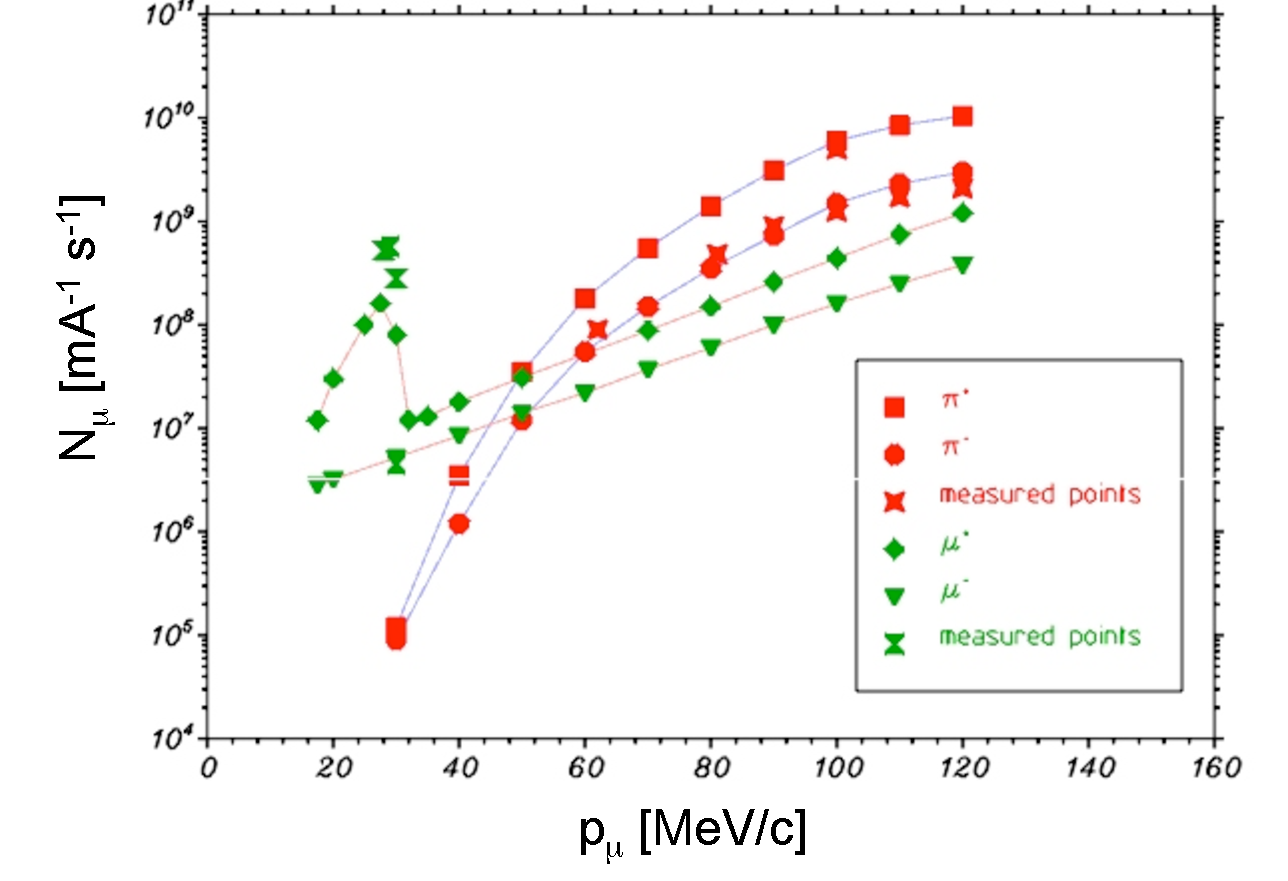
\includegraphics[width=0.51\textwidth]{ChargedLeptons/Figures/MuonRates.pdf}\hfill
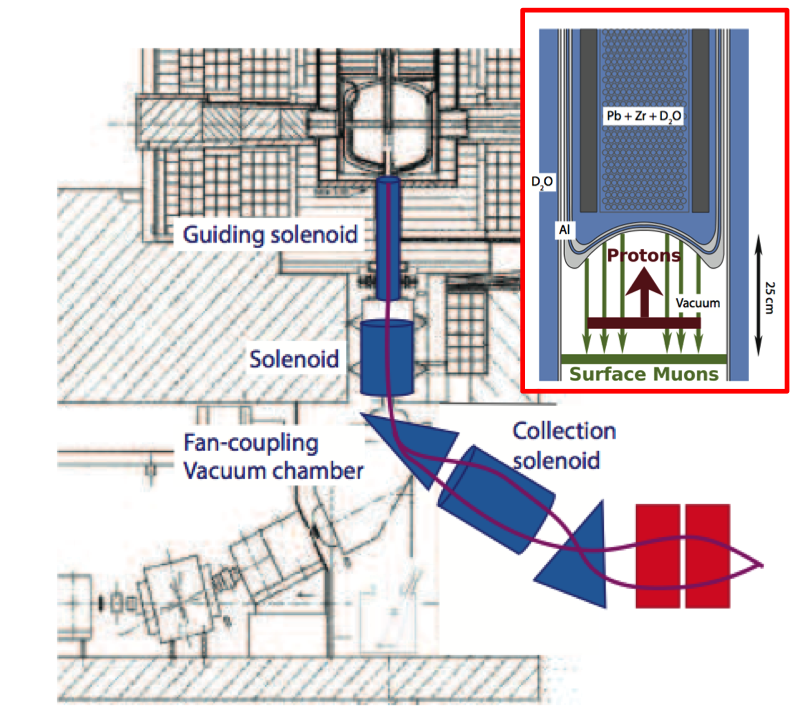
\includegraphics[width=0.46\textwidth]{ChargedLeptons/Figures/HIMB.pdf}
\caption{Left panel: Pion and muon rates versus particle momentum for both charges predicted for the $\pi$E5 beamline at PSI together with a few measured data points. Right panel: Conceptual design of a possible high intensity muon beamline at the spallation source target at PSI. Red inlet is a zoom of the neutron target region.\label{fig:cl:muonrates}}
\end{figure}

The high rates of surface (and sub-surface) positive muons and their low momentum leading to a high stopping density as explained above make these an ideal choice for the searches of CLFV via $\mu^+\to e^+ \gamma$ or $\mu^+ \to e^+ e^+ e^-$. Other physics experiments such as the MuLan experiment \cite{Tishchenko:2012ie} also relied on surface muon beams due to the high rates while employing a thin stopping target. Table \ref{table:cl:muonexperiments} shows some examples of finalized and future particle physics experiments that all use surface muons (except for the future Mu2e experiment at FNAL which requires negative muons). From the beam rates column one can see that future experiments require the next generation surface muon beams with rates of an order of magnitude larger than the current available maximum rates at PSI. 

\begin{table}[ht]
\begin{center}
\caption{Overview of some muon experiments and their beam parameters. Experiment marked with $^*$ are future experiments.\label{table:cl:muonexperiments}}
{ \begin{tabular}{lllll}\\
\hline
{\bf Experiment} & {\bf Beam} & {\bf Momentum} & {\bf Rates} & B{\bf Beamline}\\
{\bf } & {\bf } & {\bf [MeV/c]} & {\bf [s$^{-1}$]} & \\
\hline
MEG ($\mu\to e\gamma$) \cite{Adam:2013} & $\mu^+$ & 29.8 & $3 \cdot 10^7$ & $\pi$E5 at PSI\\
\hline
MuLan \cite{Tishchenko:2012ie} & $\mu^+$ & 29.8 & $8 \cdot 10^6$ & $\pi$E3 at PSI\\
\hline
TWIST \cite{Hillairet:2012} & $\mu^+$ & 29.8 & $<5 \cdot 10^3$ & TRIUMF\\
\hline
MEG upgrade$^*$ ($\mu\to e\gamma$) \cite{Baldini:2013ke} & $\mu^+$ & 29.8 & $7 \cdot 10^7$ & $\pi$E5 at PSI\\
\hline
Mu2e$^*$ ($\mu^- \to e^-$) \cite{Abrams:2012er} & $\mu^-$ & $\sim 40$ & $10^{10}$ & FNAL\\
\hline
$\mu^+ \to e^+e^-e^+$ (Phase 1)$^*$ \cite{Blondel:2013ia} & $\mu^+$ & $29.8$ & $<1 \cdot 10^8$ & $\pi$E5 at PSI\\
\hline
$\mu^+ \to e^+e^-e^+$ (Phase 2)$^*$ \cite{Blondel:2013ia} & $\mu^+$ & $29.8$ & $2 \cdot 10^9$ & HIMB at PSI\\
\hline
\end{tabular}}
\end{center}
\end{table}

In addition to the listed particle and nuclear physics experiments in Table \ref{table:cl:muonexperiments}, surface muon beams are highly polarized making them very suitable for material science applications via the Muon Spin Rotation (muSR) technique. Several facilities worldwide currently provide surface muon beams. Table \ref{table:cl:muonrates} shows the two laboratories (PSI, J-PARC, and RCNP Osaka University) with the currently highest rates of up to a few $10^8$\,s$^{-1}$ as well as future estimated rates including a possible facility at Fermilab with Project-X beams. Other facilities like TRIUMF, KEK, RAL-ISIS, and Dubna have rates $< 10^7$ \,s$^{-1}$ and were omitted in this table.

\begin{table}[ht]
\begin{center}
\caption{Summary of some current and planned muon beam facilities at various worldwide laboratories. Table reproduced in parts from \cite{Blondel:2013ia} \label{table:cl:muonrates}}
{ \begin{tabular}{llll}\\
\hline
Laboratory / & Energy / & Present Surface  & Future estimated  \\
Beam Line & Power & $\mu^{+}$ rate (Hz) & $\mu^{+}/\mu^{-}$ rate (Hz) \\
\hline
\bf{PSI (CH )} & (590 MeV, 1.3 MW, DC) &  & \\
LEMS & `` & $4 \cdot 10^8$ &  \\
$\pi$E5 & `` & $1.6 \cdot 10^8$  & \\
HiMB & (590 MeV, 1 MW, DC) & & $4\cdot 10^{10} (\mu^{+})$ \\
\hline
\bf{J-PARC (JP)} & (3 GeV, 1MW, Pulsed) & & \\
 & currently 210 KW &  & \\
 MUSE D-line & `` & $3 \cdot 10^7$ & \\
 MUSE U-line & `` &  & $2\cdot 10^8 (\mu^{+})(2012)$ \\
 COMET & (8 GeV, 56 kW, Pulsed) & & $10^{11} (\mu^{-})(2019/20) $\\
 PRIME/PRISM & (8 GeV, 300 kW, Pulsed ) & & $10^{11-12}(\mu^{-}) ( > 2020)$ \\
 \hline
 \bf{FNAL (USA)} & &  & \\
 Mu2e & (8 GeV, 25 kW, Pulsed) & & $5\cdot 10^{10} (\mu^{-})(2019/20) $\\ 
 Project X Mu2e & (3 GeV, 750 kW, DC to pulsed) & & $2\cdot 10^{12} (\mu^{-})(>2022)$ \\
\hline 
\end{tabular}}
\end{center}
\end{table}

Next generation CLFV experiments with a surface muon beam ($\mu^+ \to e^+\gamma$ \cite{Baldini:2013ke} and $\mu^+ \to e^+e^-e^+$ \cite{Blondel:2013ia}) are in the design and planning stages at PSI. Since these experiments have to suppress accidental backgrounds which scale with the square of the beam rate, they require continuous beams. The current $\pi$E5 beamline at PSI with conventional focusing quadrupole elements can deliver about $2\cdot10^8$\,muons/s at the proton beam power of 1.3\,MW. However, this beamline views target station E \cite{Heidenreich:2002zz} at PSI where only about 20\,\% of the proton beam interacts. Most of the beam is transmitted to the neutron spallation target at the end of the proton beamline. PSI is currently studying the possibility of a high instensity muon beamline (HIMB) at the neutron spallation target based on a large capture solenoid concept. The conceptual design is shown in the right panel of Figure \ref{fig:cl:muonrates}. About 70\,\% of the 1.3 MW proton beam is coming from the left and directed upwards into the SINQ target of lead-filled zircaloy tubes surrounded by a cooling D$_2$O layer. Surface muons from the aluminum window (see red framed inlet) could then be collected in the downwards direction with newly installed solenoids (blue) into a new dedicated new beamline. Realistic Monte Carlo simulations give an estimate of about $1\cdot10^{11}$\,muons/s below 29.8\,MeV/c corresponding to a rate of $3\cdot 10$\,s$^{-1}$ for 10\,\% momentum bite around 28\,MeV/c \cite{Blondel:2013ia}.

Table \ref{table:cl:muonrates} also shows the different beam energies at the 3 facilities. While PSI employs a DC, 590\,MeV proton beam of about 1.3\,MW total power, J-PARC (pulsed mode) and Fermilab with its future Project-X\footnote{http://projectx.fnal.gov/} accelerator infrastructure (DC and pulsed mode) have 3\,GeV beams eith about 1\,MW of power. Original studies at ISIS \cite{Bungau:2013hd} found that the muon yields per MW of beam power are 3-7 times lower at 3\,GeV compared to PSI's 590\,MeV. However, recently corrected pion cross sections in GEANT4 demonstrated that the yields are rather similar \cite{striganov:12}. Therefore, an optimized surface muon beamline in the Project-X era at Fermilab with 750\,kW beam power could be a competetive option to a HIMB development at PSI. 

As described in the following sections, the feasibility of next generation experiments ($\mu^+ \to e^+\gamma$ and $\mu^+ \to e^+e^-e^+$) would require the availability of a high rate (sub-)surface muon beam. With the prospect of the high power 3\,GeV beams at Project-X surface muon beams could become available to a multitude of applications at Fermilab such as particle physics and material science with muSR. Besides the available beam power of about 750\,kW for a muon program, the flexibility of the accelerator beam structure is an additional benefit to serve a multitude of experiments with different requirements. The design of a future surface muon beamline will need to take into account a variety of parameters for the optimization:
\begin{itemize}
\item Proton target: The design of the proton target by itself has many design parameters. The target can either be at the end of the proton beamline in conjunction with a planned neutron spallation target similar to aforementioned HIMB strategy at PSI. Alternatively, the proton target could be in the proton beam and only using a fraction of the available beam. The material choice and target shape influence the surface muon yields, mechanical stability and determine the cooling requirements. Other aspects of the design include the minimization of secondaries (e.g. $e^\pm$, $\pi^\pm$, $\gamma$, and $n$) and ideally a low activation throughout operation. 
\item Muon beam channel: The development of a specific concept of the muon beam channel should be based on the experimental requirements such as required muon rates, polarization, momentum and momentum bite as well as the beam spot at the stopping target. As mentioned before, there are two major concepts based on either a more conventional design with focusing quadrupole elements or large solid angle capture solenoids. Specific elements such as a $E\times B$ separator will influence the beam contamination with electrons and the length of the beamline and pulsed mode are important for the remaining pion flux.
\item The muon stopping target: While this element is not necessarily part of the beam channel design, it is yet necessary to include its optimization together with the available tuning parameters of a beamline (such as momentum, momentum bite and beam spot). Design parameters include the target material and shape. 
\end{itemize}

Alternatively to a dedicated new surface muon beamline(s) at Project-X that could serve both the next generation particle physics experiments and a muSR user community, one should also investigate in more details whether the future Mu2e proton target and capture solenoids could be adapted for a surface muon beam. Very first Monte Carlo simulations indicate that surface muons would be transported through the solenoids and might be efficiently stopped in a thin walled tubular target. For pion suppression, the Mu2e setup operates in pulsed mode which is not ideal for experiments like $\mu^+ \to e^+\gamma$ and $\mu^+ \to e^+e^-e^+$ as explained above due to the accidental backgrounds. While a simple estimate of a pulsed mode only shows a slight loss compared to an ideal DC beam, a detailed investigation with a full simulation is required to compare an adapted Mu2e beamline to a dedicated surface muon facility. In addition, the current Mu2e setup does not include a separator for electron suppression.

In summary, the prospect of a high power 3\,GeV proton beam available for a future muon program at Project-X offers the opportunity to provide a world leading surface muon beam competitive with the rates at other facilities (specifically the planned HIMB beamline at PSI). This could facilitate the next generation of CLFV experiments in addition to a material science oriented muSR facility. However, given the variety of optimization parameters, the development of a concept would require significant Monte Carlo and other design studies.

%\bibliography{ChargedLeptons/surface}
